\section{Theory}
Photomultiplier tubes (PMTs) are highly sensitive photon detectors widely employed in the detection of weak optical signals, spanning ultraviolet (UV) to visible wavelengths, as well as high-energy photons such as X-rays and gamma rays. When coupled with scintillators, PMTs are also instrumental in detecting ionizing radiation. 


The main parts of the PM tube are (ref Fig. 1) -- 
\begin{enumerate}
    \item A window (faceplate) that allows light to enter
    \item A photoemissive cathode (photocathode) followed by focusing electrodes
    \item Electron multipliers (dynodes)
    \item An electron collector (anode) within a vacuum
    tube
\end{enumerate}

The photocathode is a semitransparent thin layer of photoemissive material deposited on the inner surface of the window. When photons are absorbed, electrons are emitted. The photocathode can be configured in either a head-on or a side-on arrangement. In the head-on type, light enters through the end of the tube, while in the side-on type, it enters through the sides.

Dynodes are coated with a secondary emissive material. Each incident electron on a dynode releases multiple secondary electrons, leading to an amplification process.

The process of generation of an output signal in a PMT is detailed below.

\begin{itemize}
    \item Incident light passes through the glass window and excites electrons in the photocathode, causing the emission of photoelectrons into the vacuum (external photoelectric effect)
    \item The emitted photoelectrons are directed by focusing electrodes and accelerated towards the first dynode, where secondary electron emission occurs.
    \item The secondary electrons are accelerated towards the next dynode by an inter-dynode potential, typically around 100 V, producing additional secondary electrons. The required electrode potentials are generally supplied by a high-voltage source and regulated through a resistive or transistorized voltage divider.
    \item This process of secondary electron emission is repeated at successive dynodes.
    \item The final cluster of secondary electrons, amplified up to a factor of 103 to 108 depending on the number of dynodes and inter-dynode potentials, is collected at the anode, generating an output signal.
\end{itemize}

\begin{figure}
    \centering
    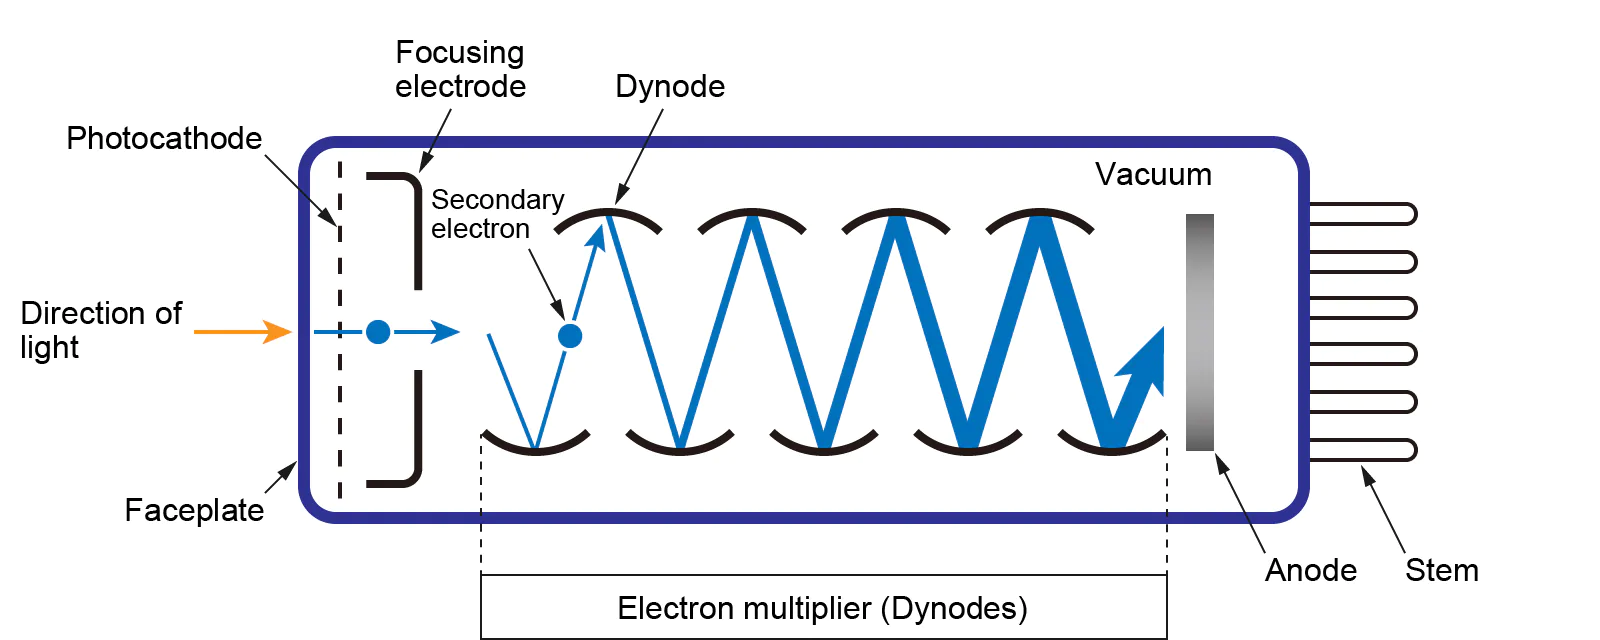
\includegraphics[width=1\columnwidth]{images/pmt.png}
    \caption{Construction of a photomultiplier tube}
    \label{g1}
\end{figure}

\subsection{PMT Characteristics}

\subsubsection{Current Gain}
Electrons emitted from the photocathode are accelerated under the electric field and go to the first dynode and emit a secondary electron that hits the next dynode again emitting a secondary electron.Repeating this process over successive dynode stages achieves a high current amplification. So for a small value of current from photocathode gives rise to a large output current. The current amplification of a PMT is defined as the ratio of the anode output current to the photoelectric current from the photocathode. Ideally, for a photomultiplier tube with $n$ dynode stages and an average secondary emission ratio $\delta$ per stage, the total current amplification is given by:
\begin{align}\mu = \delta^n\end{align}
The secondary electron emission ratio $\delta$ is expressed as:
\begin{align}\delta = AE^\alpha\end{align}
where $A$ is a constant, $E$ is the interstage voltage, and $\alpha$ is a coefficient determined by the dynode material and its geometric structure, typically ranging from 0.7 to 0.8. When a voltage V is applied between the cathode and anode of a PMT with $n$ dynode stages, the current amplification $\mu$ becomes:
\begin{align}
    \mu &= \delta^n \nonumber\\ 
    &=(AE^\alpha)^n\nonumber\\
     &=A\left(\frac{V}{n+1}\right)^{\alpha n}\nonumber\\ 
     &=K'V^{\alpha n}
\end{align}
Since PMTs typically have 9 to 12 dynode stages, the value of $n \alpha$ generally falls within the range of 6 to 10.

\subsubsection{Voltage Gain}
The voltage gain G of a PMT is defined as the ratio of the output voltage to the input voltage at a particular applied voltage V (at constant supply voltage V) \begin{align}G = \frac{V_{out}}{V_{in}}\end{align}

Experimentally, voltage gains $G_1$ and $G_2$ can be measured at applied voltages $V_1$ and $V_2$, respectively, satisfying the relation
\begin{align}\frac{G_1}{G_2} = K\left(\frac{V_1}{V_2}\right)^{n\alpha}\end{align}

\subsubsection{Dark Current}
Even in the absence of incident light, a small current can still be observed in a photomultiplier tube. This residual current, known as the anode dark current, contributes to noise and affects the overall detectivity of the PMT.

The dark current strongly depends on the applied supply voltage. The primary sources of dark current include:

\begin{itemize}
    \item Spontaneous emission of electrons due to thermal energy
    \item Ionization of residual gases within the vacuum tube
    \item Electron emission due to strong electric fields at sharp point
    \item Small leakage currents arising from imperfections in insulation
    \item Light emission caused by interactions with the glass envelope
\end{itemize}
These factors collectively contribute to the overall dark current, and their minimization is crucial for improving the sensitivity of the photomultiplier tube.

\subsection{Spectral Response}

The efficiency of a photomultiplier tube in converting incident photons into emitted electrons depends on the photocathode’s sensitivity, which varies with wavelength. This dependency is referred to as the spectral response characteristic. 

The spectral response is primarily influenced by two key factors.

The long-wavelength limit is determined by the composition of the photocathode material, which governs its ability to release electrons upon photon absorption.

The short-wavelength limit is dictated by the optical properties of the input window material, as certain materials absorb high-energy (short-wavelength) photons before they can reach the photocathode.

Understanding these spectral response characteristics is essential for selecting an appropriate PMT for specific applications, ensuring optimal sensitivity across the desired wavelength range.

% ======================================================================================
\section{Experimental Setup}

\subsection*{Apparatus}

\begin{enumerate}
    \item PMT Module (H9305-03)
    \item  Control voltage unit
    \item  Digital Storage Oscilloscope(DSO)
    \item  Tungsten filament bulb
    \item  DC power supply
    \item  Optical Filters for different wavelengths (in the
    range 400 – 700 nm) with a suitable holder
    \item  Mounted photodiode
    \item  Multimeters
    \item  Breadboard and Connecting cables
\end{enumerate}

\begin{figure}[H]
    \centering
    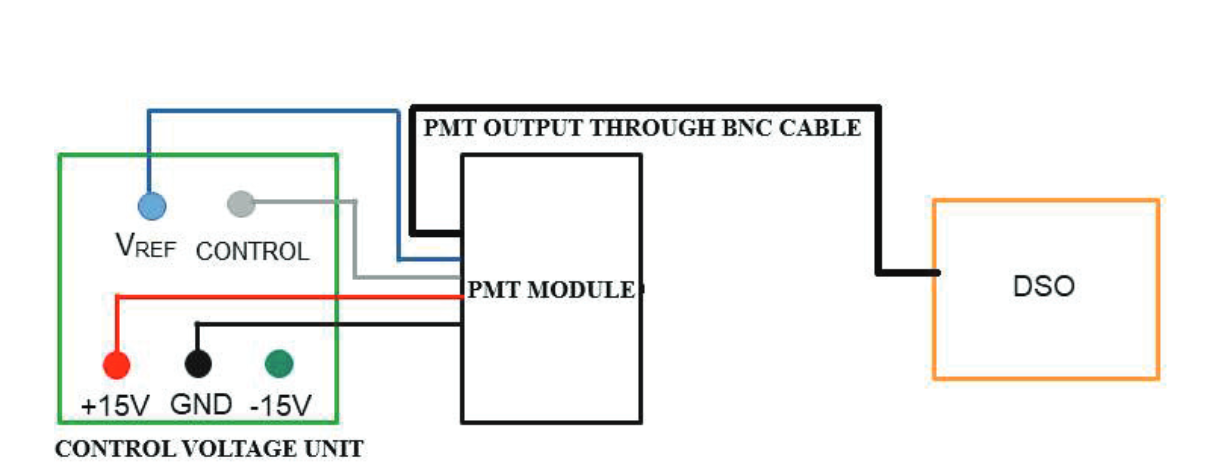
\includegraphics[width=1\columnwidth]{images/circ.png}
    \caption{Schematics of Connections of PMT module to control voltage unit}
    \label{g1}
\end{figure}